
\begin{figure}
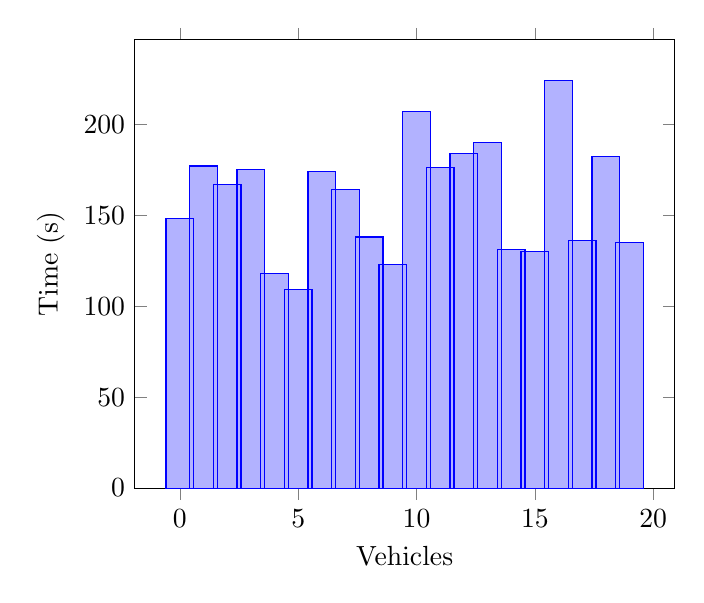
\begin{tikzpicture}
\begin{axis}[
legend style={anchor=west},
xlabel=Vehicles,
ylabel=Time (s),
ymin=0,
ybar,
]
\addplot coordinates {
(0, 148)
(1, 177)
(2, 167)
(3, 175)
(4, 118)
(5, 109)
(6, 174)
(7, 164)
(8, 138)
(9, 123)
(10, 207)
(11, 176)
(12, 184)
(13, 190)
(14, 131)
(15, 130)
(16, 224)
(17, 136)
(18, 182)
(19, 135)
};

\end{axis}
\end{tikzpicture}
\label{tik:0:3_V, 3_V.-60, 4_S, 5_S, 5_S.-30, 7_S, 7_S.-25, 11_S, 11_S.-50, 13_S, 15_N, 17_S, 17_S.-60, 19_V}
\caption{0 percent diving with GSC on route $3_V, 3_V.-60, 4_S, 5_S, 5_S.-30, 7_S, 7_S.-25, 11_S, 11_S.-50, 13_S, 15_N, 17_S, 17_S.-60, 19_V$}
\end{figure}
